\section{Feature Engineering}
Features are the fundamentals for machine learning task. For text data, basic
features include meta-data (author, publish year, organizations), topic
distributions (latent topics of document), and word features. For different type
of features, there are different methods to transfer them to numerical values.

\subsection{Meta-data}
Meta-data is useful for modeling text. I would use index map to encode
meta-data. First of all, I would set every meta-data with a index. Then for each
publication, if the meta-data appeared, I would set the feature index as 1,
otherwise 0. Meta-data include:

\begin{enumerate}[a]
\item \textbf{Authors.} authors are very important attributes of a
paper. I can use an indicator vector to encode this attribute to a vector as
input feature. At first, I assign every different author a index. Then for each
paper, I would put 1 to the position of the index for every author in the paper,
otherwise 0.

\item \textbf{Organizations.} similar to authors.

\item \textbf{Time.} time is also very import attribute for a paper. The research
topics of a conference would change over time. Therefore, when predicting
conference for a paper, I need to take the time into consideration. I could use
the year as the input of the feature.
\end{enumerate}

\subsection{Topic Distributions}
When researchers are writing publications, they would first set the hidden topics
that publications would cover. If we could well model the hidden topic
distributions, then we could naturally model the topic distributions of
conferences via modeling publications it contained.

\subsubsection{LDA}
LDA is commonly used to mine the latent topic distributions
of documents \cite{blei2003latent} \cite{griffiths2004finding}.

\begin{figure}[!htbp]
    \centering
    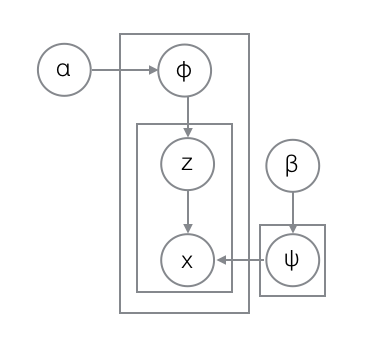
\includegraphics[width=4cm]{./pic/LDA.png}
    \caption{LDA}
\end{figure}


\begin{align*}
   & \phi_d \sim Dir (\alpha) \qquad \psi_k \sim Dir (\beta) \\
   & z_{dn} \sim Mult (\phi_x) \quad x_{dn} \sim Mult (\psi_{z_{dn}})
\end{align*}

\subsubsection{Neural Networks Upstream Conditioning LDA}
Besides traditional LDA, we could use Neural Networks Upstream Conditioning model
to mine topic distributions \cite{mimno2012topic}. The advantage of upstream
conditioning model is this method could integrate meta-data into the latent
topic distributions.

\begin{figure}[!htbp]
    \centering
    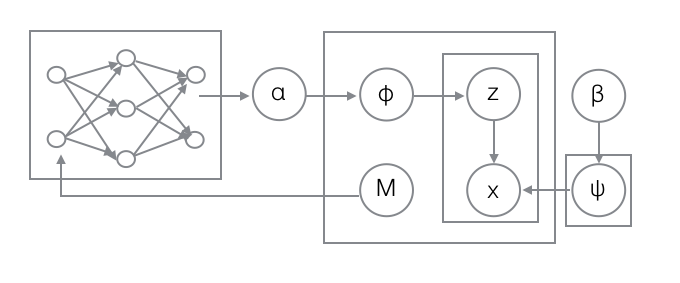
\includegraphics[width=8cm]{./pic/Up.png}
    \caption{Neural Networks Upstream Conditioning LDA}
\end{figure}

\begin{align*}
   & \alpha \sim F(M \mid W) \\
   & \phi_d \sim Dir (\alpha) \qquad \psi_k \sim Dir (\beta) \\
   & z_{dn} \sim Mult (\phi_x) \quad x_{dn} \sim Mult (\psi_{z_{dn}})
\end{align*}

\subsection{Word Features}
Word features are the most import feature for modeling documents. We have two
common ways to encode word features. The first is just use the word indicator
map, which are always used by Naive Bayes. Another way is to use word2vec, which is
a deep learning method to encode word features \cite{mikolov2013distributed}.
